\documentclass[hidelinks,12pts]{article}
\usepackage[export]{adjustbox}
\usepackage{amsmath}
\usepackage{amssymb}
\usepackage[title,titletoc]{appendix}
\usepackage{array}
\usepackage[english]{babel}
\usepackage{bbm}
\usepackage{blindtext}
\usepackage{bookmark}
\usepackage{booktabs}
\usepackage{cancel}
\usepackage{caption}
\usepackage{csquotes}
\usepackage{enumerate}
\usepackage{enumitem}
\usepackage{epigraph}
\usepackage[left]{eurosym}
\usepackage{float}
\usepackage[bottom]{footmisc}
\usepackage[margin=0.9in]{geometry}
\usepackage{graphicx}
\usepackage{hyperref}
\usepackage{indentfirst}
\usepackage{listings}
\usepackage{lscape}
\usepackage{mathtools}
\usepackage{mdframed}
\usepackage{multirow}
\usepackage{multicol}
\usepackage[sort]{natbib}
\usepackage{parskip}
\usepackage{setspace}
\usepackage{subcaption}
\usepackage{titlesec}
\usepackage{tgpagella}
\usepackage{varwidth}
\usepackage{verbatim} %comment block
\usepackage{wrapfig}
\usepackage[dvipsnames]{xcolor}
\usepackage{xltabular}

\renewcommand{\epigraphsize}{\normalsize}
\setlength{\epigraphwidth}{0.7\textwidth}
\renewcommand{\textflush}{flushright}
\renewcommand{\sourceflush}{flushright}


\renewcommand\appendixpagename{Mathematical Appendix}
\renewcommand{\baselinestretch}{1.45}

\hypersetup{
    colorlinks=true, 
    urlcolor= Violet, 
    linkcolor=Black, 
    citecolor=Blue, 
    filecolor = Blue
    } 

%\usepackage{natbib}
\bibliographystyle{plainnat}
%\bibdata{My Library.bib}
%\usepackage[backend=biber, style=authoryear-icomp]{biblatex}

\DeclareMathOperator{\E}{\mathbb{E}}
\DeclareMathOperator{\Prb}{\mathbb{P}}
\DeclareMathOperator{\R}{\mathbb{R}}
\DeclareMathOperator{\N}{\mathbb{N}}
\DeclareMathOperator{\1}{\mathbbm{1}}
\newcommand{\ind}{\perp\!\!\!\!\perp}


\titleformat{\part}{\centering\normalfont\Large\bfseries}{\partname\hspace{5pt}\thepart\hspace{5pt}}{5pt}{--\ }

\titleformat{\part}{\centering\normalfont\Large\bfseries}{\partname\hspace{5pt}\thepart\hspace{5pt}}{5pt}{--\ }

\makeatletter
\def\@fnsymbol#1{\ensuremath{\ifcase#1\or \dagger\or \ddagger\or
   \mathsection\or \mathparagraph\or \|\or **\or \dagger\dagger
   \or \ddagger\ddagger \else\@ctrerr\fi}}
    \makeatother

%code snippets 
\definecolor{codegreen}{rgb}{0,0.6,0}
\definecolor{codegray}{rgb}{0.5,0.5,0.5}
\definecolor{codepurple}{rgb}{0.58,0,0.82}
\definecolor{backcolour}{rgb}{0.95,0.95,0.92}

\lstdefinestyle{mystyle}{
    backgroundcolor=\color{backcolour},   
    commentstyle=\color{codegreen},
    keywordstyle=\color{magenta},
    numberstyle=\tiny\color{codegray},
    stringstyle=\color{codepurple},
    basicstyle=\ttfamily\footnotesize,
    breakatwhitespace=false,         
    breaklines=true,                 
    captionpos=b,                    
    keepspaces=true,                 
    numbers=left,                    
    numbersep=5pt,                  
    showspaces=false,                
    showstringspaces=false,
    showtabs=false,                  
    tabsize=2
}

\lstset{style=mystyle}



\begin{document}

        \title{\scshape{Financial Econometrics 1 - M2 FTD \\ Empirical Applications}}
        \author{Luis Miguel Fonseca \\ Stéphane Eloundou Mvondo\\ Natalia Cárdenas Frías }
        \date{\today}
        \maketitle 

\tableofcontents
\newpage


\section*{Introduction} \addcontentsline{toc}{section}{\protect\numberline{}Introduction}
\textcolor{blue}{something, probably describe how all applications make sense one after the other and what is the research question we could have made ourselves when doing the applications, try to give a coherent look to the whole thing.}

This document compiles all our applications for the Financial Econometrics course. 
Each section represents a specific application, but we tried to make them coherent across them around a broad question: 





\section{Series Dynamics}\label{sec:dynamics}

\textcolor{gray}{\emph{Note:} Depending on each exercise along these applications we might use different series. In this first section, we performed the stationarity and component analysis of all of them to be able to use them rapidly without having to worry about seasonality or the presence of UR. Therefore, this section encompasses more than the 3 series that were asked in the exercise.}


In this work, we focus on the US market.
We use the following series retreived for the most part from FRED with its Python API (FRED tickers are in square brakets) : 

\paragraph{Inflation Expectation [MICH]}
This data series is made public by the University of Michigan from their Survey of Consumers. 
The series represent the median expected value of the percent change in prices over teh next year. 
The series is not seasonally adjusted.


\paragraph{GDP deflator [A191RI1Q225SBEA]}  
As a measure of inflation, we decided to use the implicit price deflator of teh US GDP. 
Unlike measures like the CPI deflators do not consider baskets of goods and therefore are broader measures of the price changes across all the economy that measure teh ratio of the GDP in value and in volume. 
It is a measure produced by the US Bureau of Economic Analysis as a quaterly measure in percent change QoQ. 
The raw series is already seasonally adjusted at an annual rate. 


\paragraph{Unemployment rate [UNRATENSA]}
It represents the share (in percent) of unemployed people over the labor force \footnote{The labor force data in this context encompasses people older than 16, living in continental US, who don't reside in institutions like prisons or homes for the aged, and who are not in active duty in the military.}. 
The source is the 'Current Population Survey (Household Survey)' of the US Bureau of Labor Statistics


\paragraph{FED func rate}

\paragraph{S\&P 500 price}

\paragraph{Corporate Debt Returns [BAMLCC0A0CMTRIV]}
The series represents the total returns of the debt index ICE Bank of America US Corporate Index value. 
This capitalization-weighted index tracks the performance if teh following debt instruments\footnote{Taken from the \href{https://fred.stlouisfed.org/series/BAMLCC0A0CMTRIV}{FRED's website} }: 
    \begin{itemize}
        \item[-] Of corporate debt issued in USD in the US domestic market with an investment grade rating\footnote{To be considered to have an investment grade ranking to enter the index, the company and the country must be considered investment grade by the average of the ratings of Fitch, S\&P and Moody's.}. It must have a remaining maturity of at least one year, a fixed-coupon and an outstanding amount of at least 250 million dollars.
        \item[-] Of original zero-coupon bonds ussued simultaneously in the US and the Eurobond market. 
        \item[-] Of 144a securities and pay-in-kind securities, including toggle notes, that can only be traded bu qualified institutional buyers with large portfolios. 
        \item[-] Of callable perpetual securities if they are at least one year from the first call date. 
        \item[-] Of fixed-to-floating rate securities if they are callable within the fixed rate period and are at least one year from the last call prior to the date the bond transitions from a fixed to a floating rate security. 
    \end{itemize}

The data's source is ICE Data Indices, and it is a daily series with close prices.
It is not seasonally adjusted. 





All (monthly\footnote{One should adapt the number of indicators in the seasonal components according to the data frequency.}) time series de can be decomposed in the following elements: 
    \begin{equation*}
        X_t =  \underbrace{\alpha}_{\text{drift}} + \underbrace{\beta \times t}_{\text{deterministic trend}} + \underbrace{\gamma Tt}_{\text{stochastic trend}} + \underbrace{\Sigma_{i=1}^{11} \rho_i \1_{m_i}}_{\text{seasonality}} + \underbrace{c_i}_{\text{cyclical component}}
    \end{equation*}

Remark that according to definitions, the deterministic might as well include the drift/constants $\alpha$.
Also, distinguishing the presence of a deterministic and stochastic trend needs to be done jointly and with specific procedures (see Section \ref{sec:adf} for the implementation of the ADF unit root tests). 

Using R's built-in function \texttt{stl}\footnote{Seasonal Decomposition of Time Series by Loess}, we can decompose the time series. 
The results are plotted in Figure \ref{fig:decomposition}.

\begin{figure}[h!]
    \centering
    \begin{subfigure}[b]{0.9\textwidth}
        \centering
        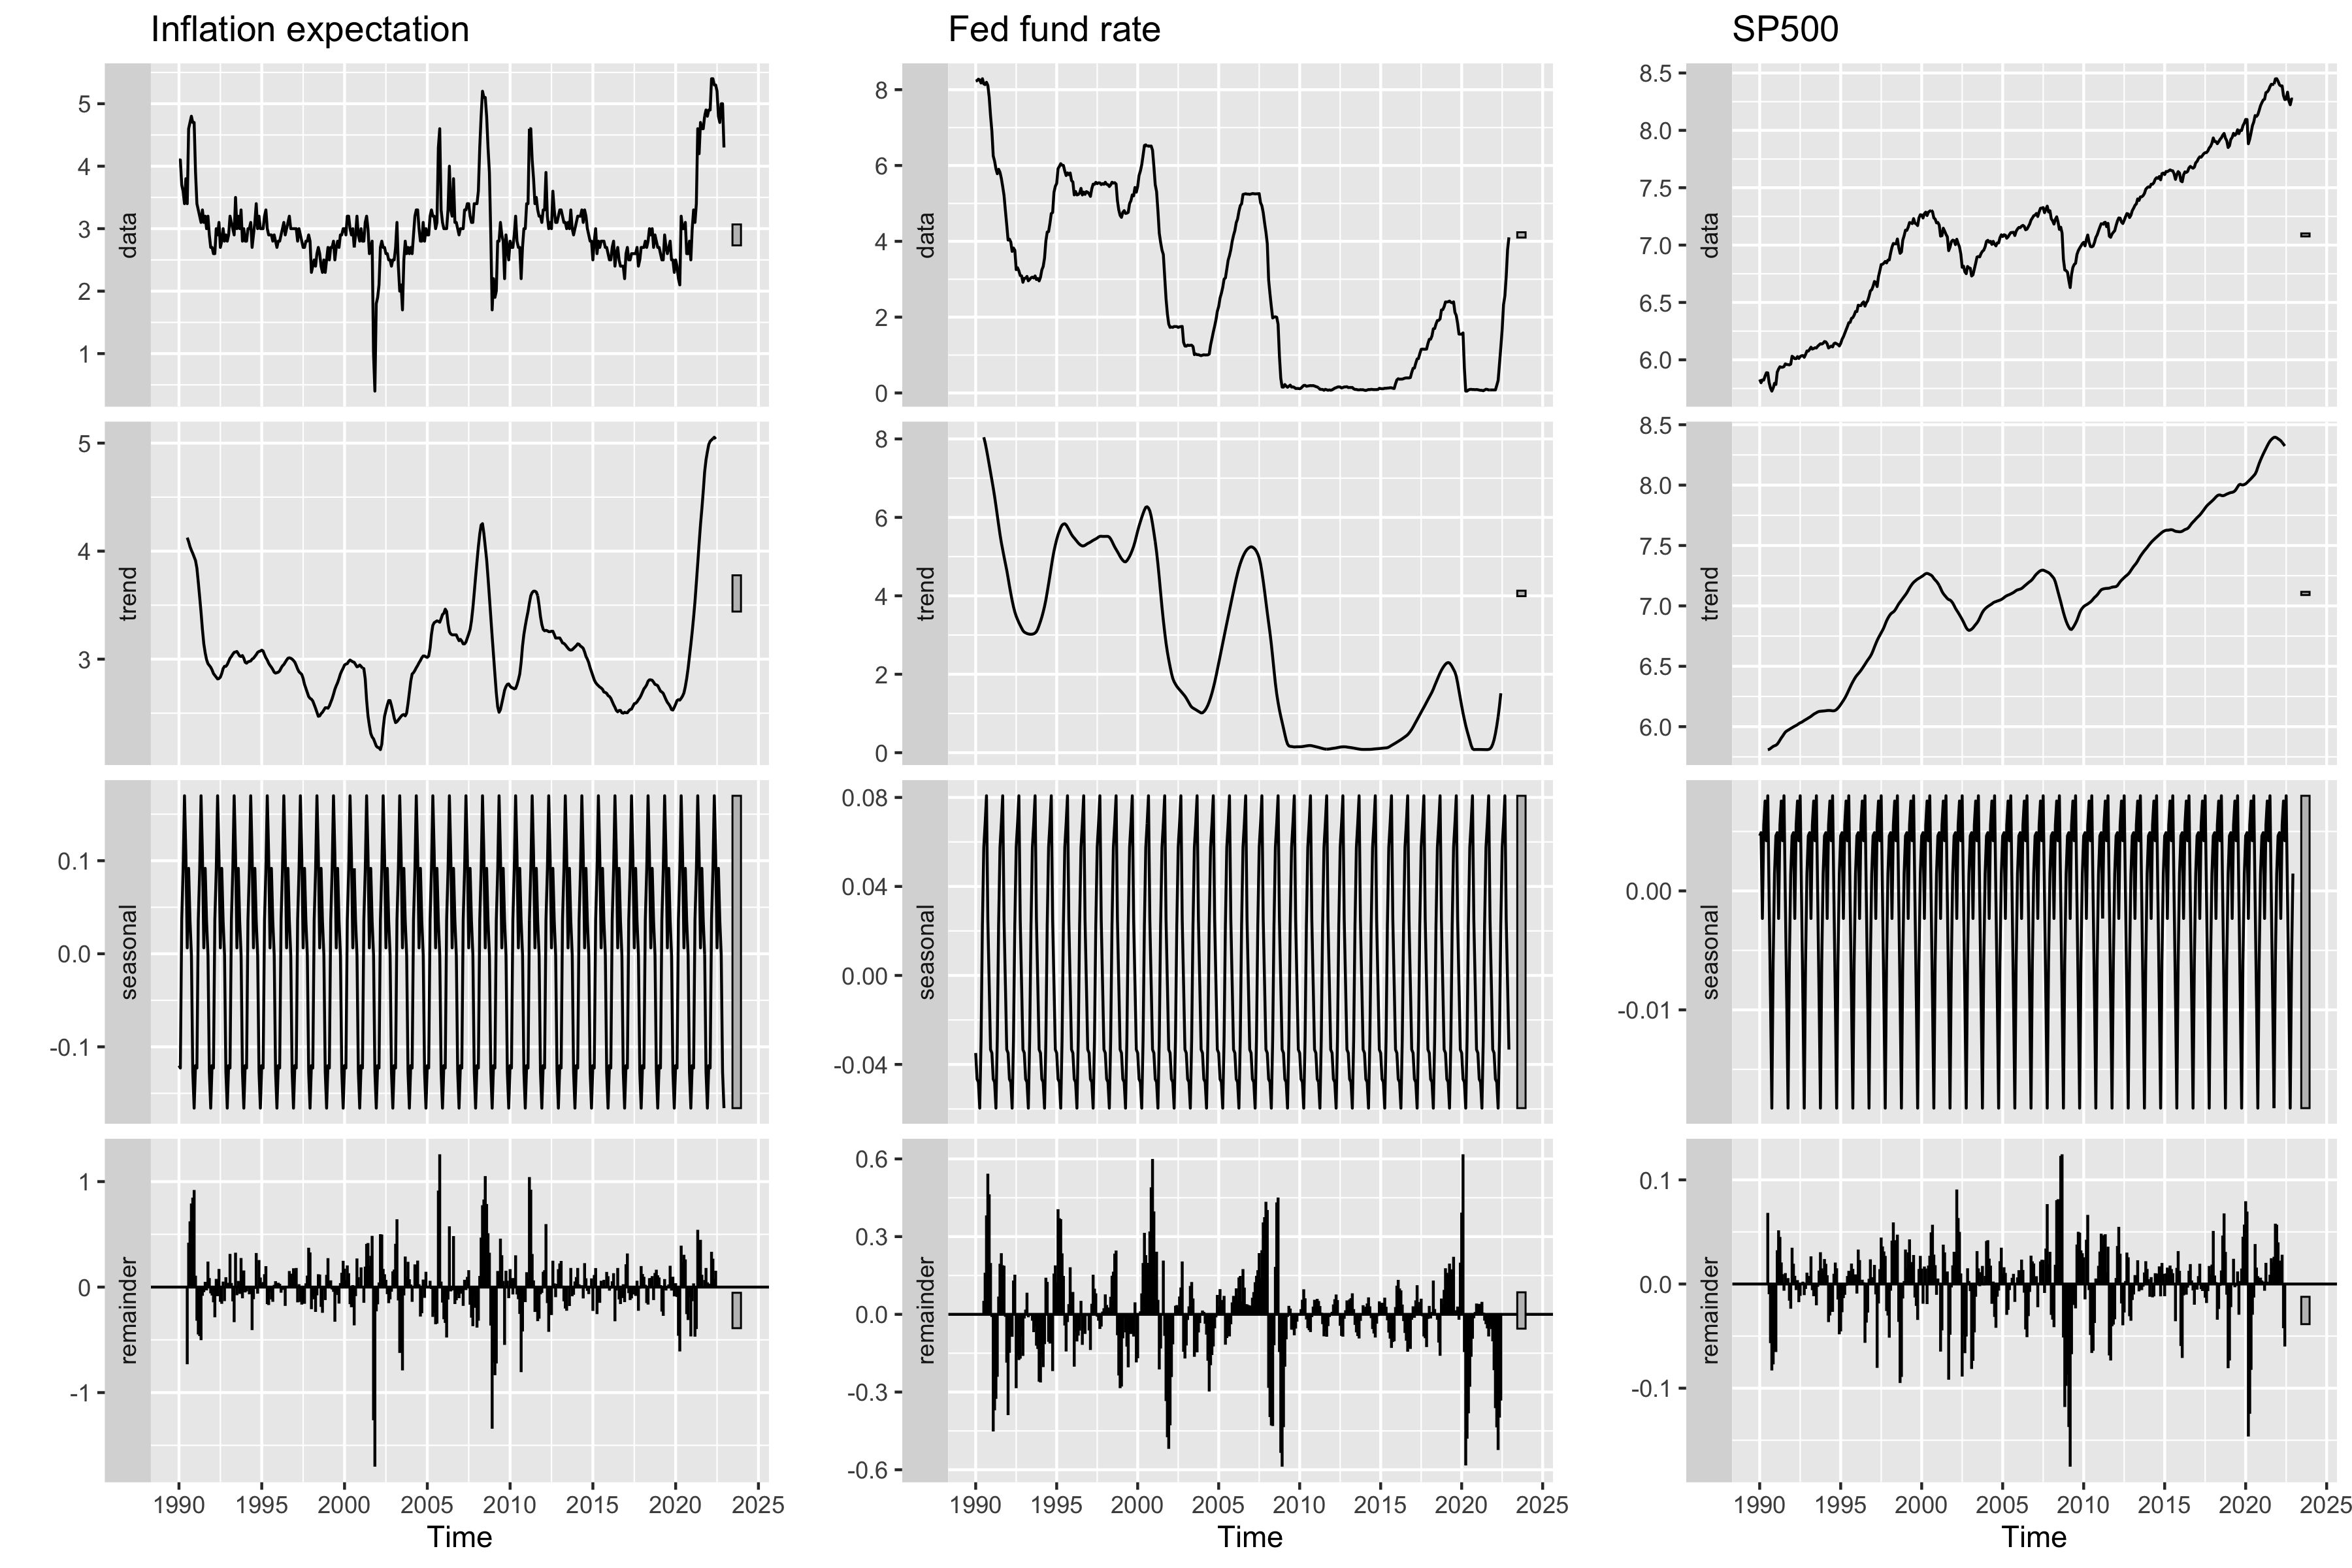
\includegraphics[width=\textwidth]{IMAGES/decomposition_i.png}
        \caption*{}
    \end{subfigure}
    \hfill
    \begin{subfigure}[b]{0.9\textwidth}
        \centering
        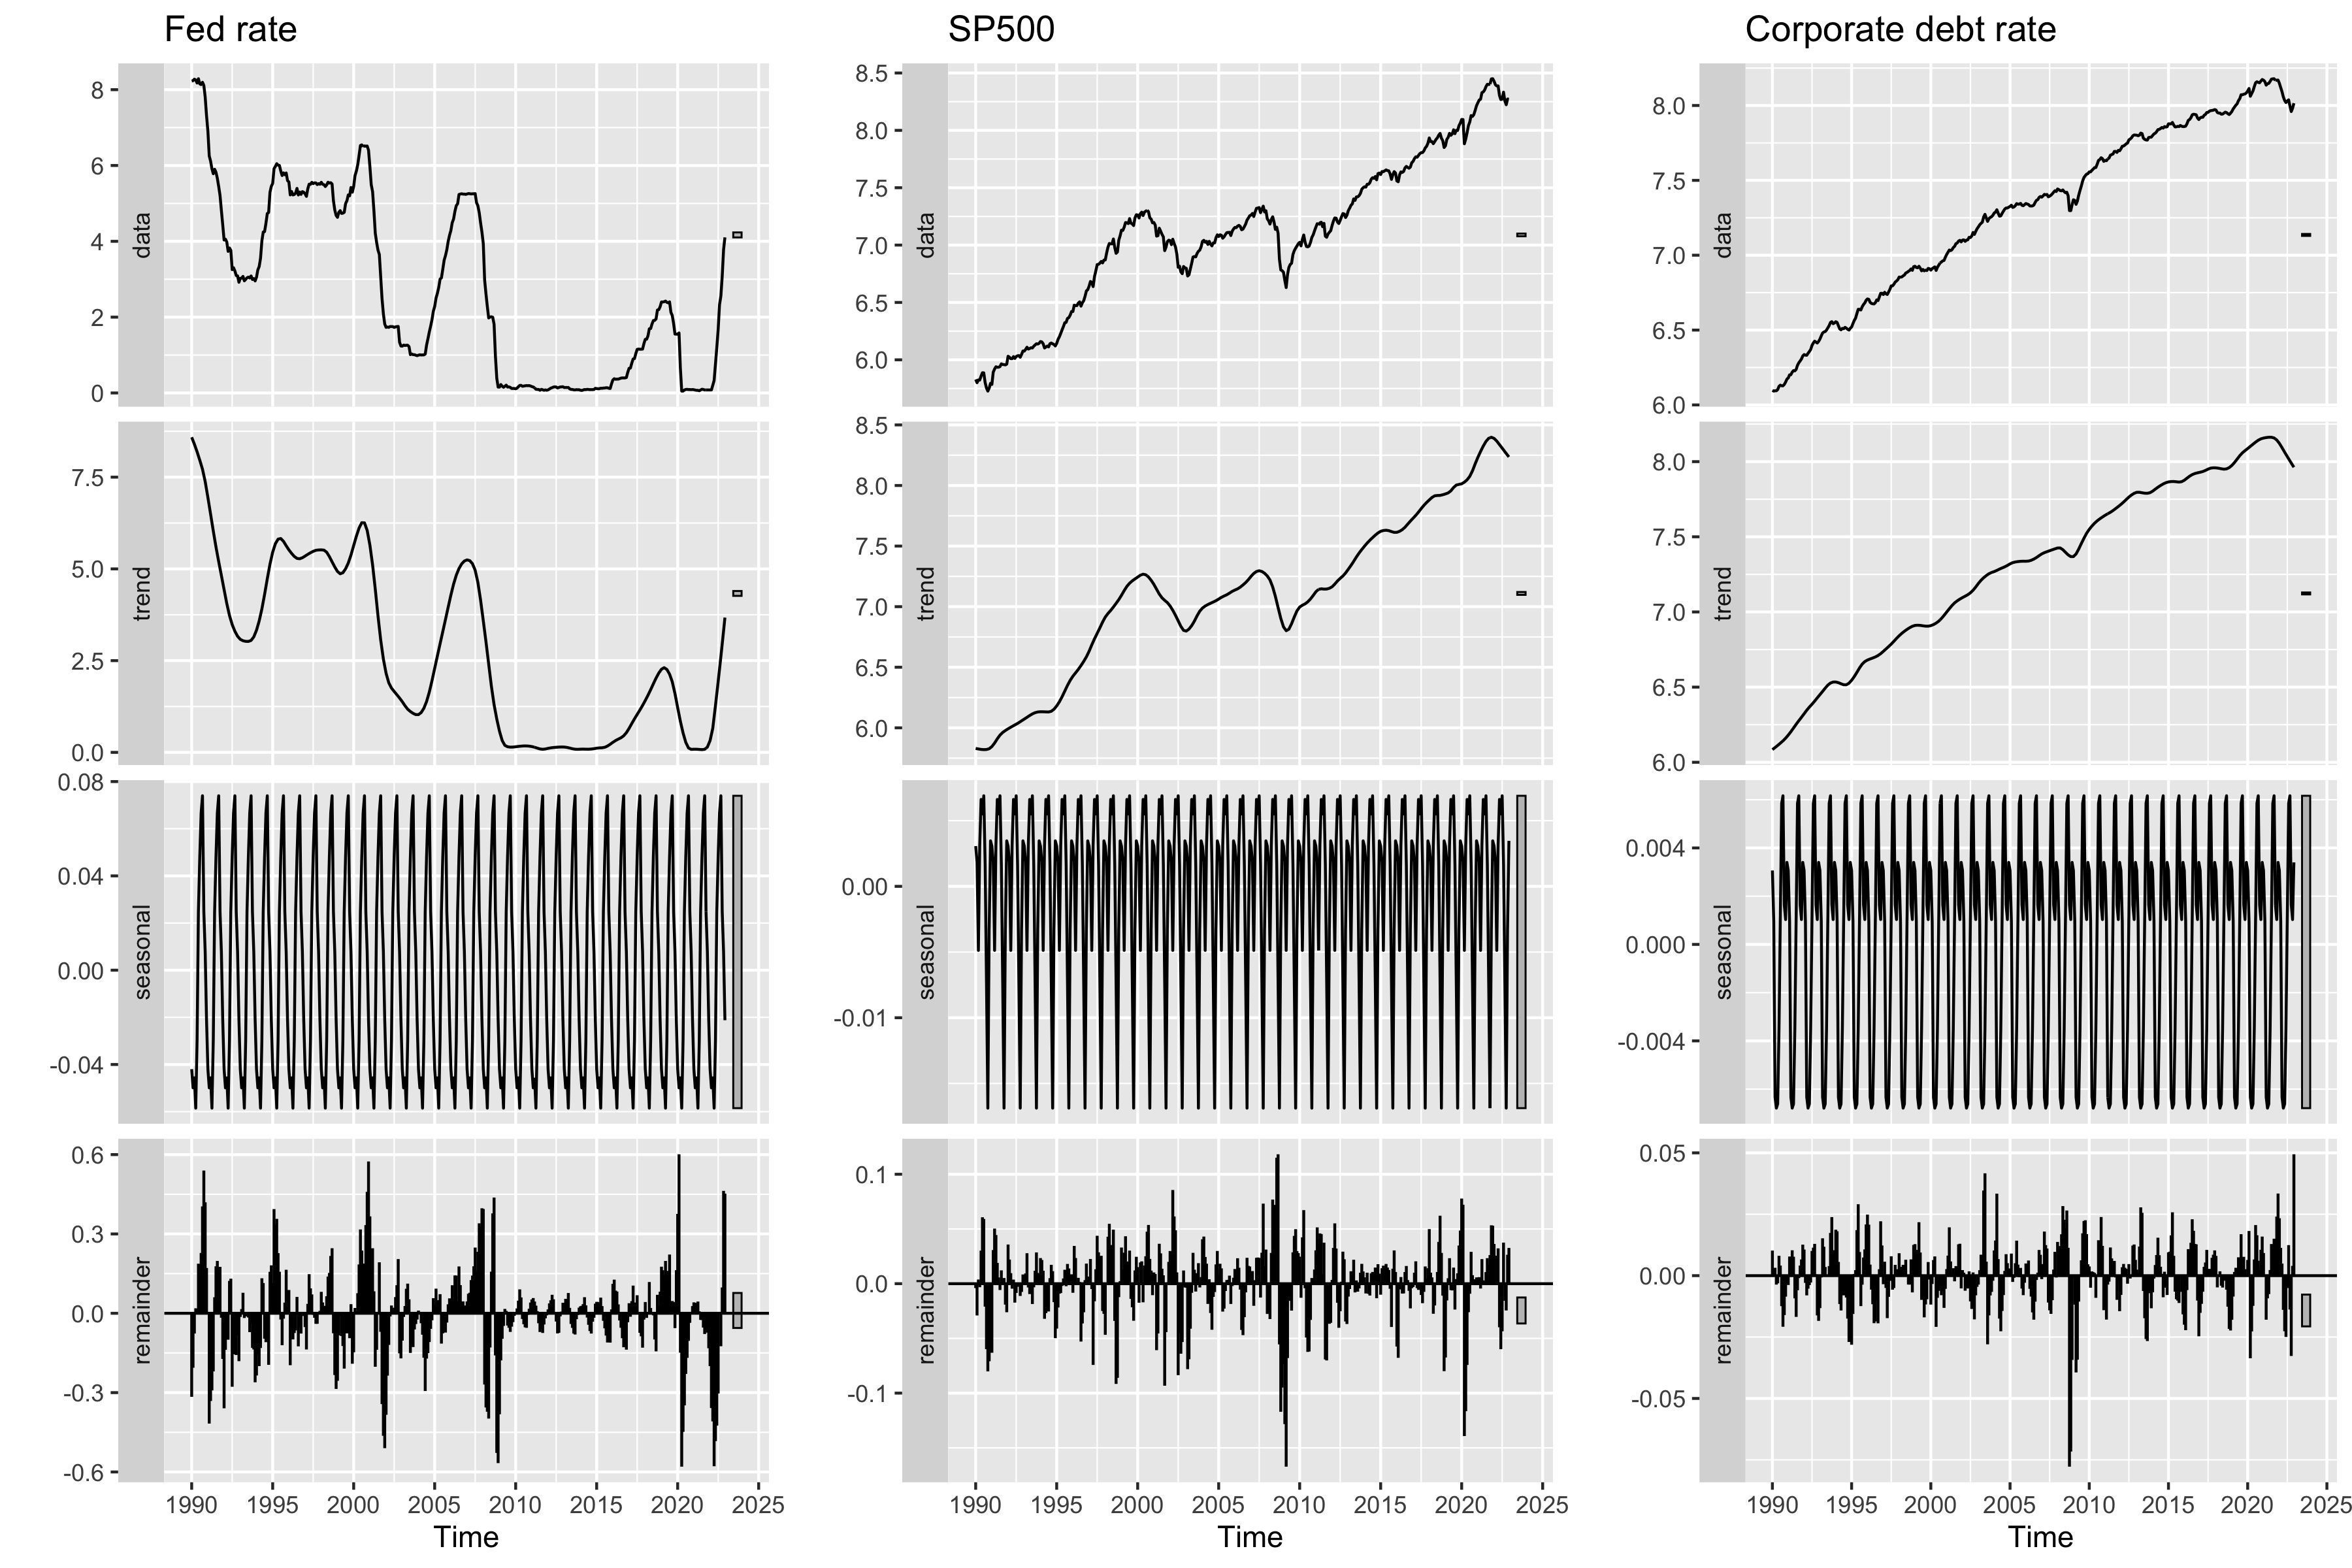
\includegraphics[width=\textwidth]{IMAGES/decomposition_ii.png}
        \caption*{}
    \end{subfigure}
    \hfill 
    \caption{Time series decomposition}
    \label{fig:decomposition}
\end{figure}







    \subsection{Seasonality} \label{sec:adf}

From the decompositions made in the previous section, in Figure \ref{fig:decomposition} we can see that R picks up small seasonal variations in each series (the values on the y-axis are rather very small). 
The estimations of the seasonal coefficients are reported in Table \ref{tab:seasons}, which indeed shows very small coefficients.
We nonetheless decided to work with deseasonalized series even if the changes are minimal.


% Table created by stargazer v.5.2.3 by Marek Hlavac, Social Policy Institute. E-mail: marek.hlavac at gmail.com
% Date and time: Tue, Dec 05, 2023 - 20:24:19
\begin{table}[!htbp] \centering 
  \caption{Estimation of the seasonality of each series} 
  \label{tab:seasons} 
\begin{tabular}{@{\extracolsep{5pt}} ccccccccccccc} 
\\[-1.8ex]\hline 
\hline \\[-1.8ex] 
 & JAN & FEB & MAR & APR & MAY & JUN & JUL & AUG & SEP & OCT & NOV & DEC \\ 
\hline \\[-1.8ex] 
infl\_e & -0.104 & -0.108 & 0.031 & 0.078 & 0.149 & 0.1 & 0.017 & 0.088 & 0.031 & 0.006 & -0.116 & -0.173 \\ 
deflator & 0.018 & 0.035 & 0.053 & 0.072 & 0.06 & 0.045 & 0.03 & -0.024 & -0.078 & -0.128 & -0.072 & -0.012 \\ 
unempl & 0.464 & 0.327 & 0.132 & -0.045 & -0.074 & 0.296 & 0.284 & 0.007 & -0.257 & -0.406 & -0.379 & -0.349 \\ 
rate & -0.042 & -0.05 & -0.046 & -0.059 & -0.03 & 0.025 & 0.048 & 0.067 & 0.074 & 0.025 & 0.008 & -0.021 \\ 
splong & 0.003 & 0.002 & -0.005 & 0.003 & 0.007 & 0.006 & 0.007 & 0.002 & -0.007 & -0.017 & -0.003 & 0.003 \\ 
corp\_debt & 0.003 & 0.001 & -0.006 & -0.007 & -0.007 & -0.004 & 0.001 & 0.006 & 0.006 & 0.002 & 0.001 & 0.003 \\ 
\hline \\[-1.8ex] 
\end{tabular} 
\end{table} 






    \subsection{Unit root and trends}

As for any time series analysis, the first analysis to perform is regarding the presence of unit roots in the series that would make them non-stationary. 
To do so, we perform the Augmented Dickey-Fuller tests that evaluate the presence of a stochastic trend (a unit root), a deterministic trend, and an intercept or drift. 
Importantly, this test requires estimating three equations/specifications because it requires investigating the joint presence of both types of trends and drift, for them to discard elements one by one. 
The inference with this test is non-standard and requires to use of corrected critical values to assess significance with the t-statistics. 



\subsubsection{ADF - Test jointly for deterministic and stochastic trend (with drift)}

We first run the following specification to the ADF test to \emph{jointly} investigate the presence of a stochastic and a determinist trend for each series $(X_t)_t$: 
    \begin{equation}
        \Delta X_t = \alpha + \beta t + \gamma X_{t-1} +\sum_{i=1,2,..}\rho_i \Delta X_{t-i} + \varepsilon_t
    \end{equation}
As per usual, the ADF test assumes H0: $\gamma =0$ i.e. a unit root exists and the series is non-stationary.
We use R's built-in function \texttt{ur.df} with \texttt{type='trend'} to get this estimation. This function gives us (i) a regression table per series and (ii) a summary table with the following test statistics: 
    \begin{itemize}
        \item[-] tau3 refers to the t-statistic associated to $\gamma =0$ 
        \item[-] phi2 refers to the F-statistic associated to $\alpha = \beta = \gamma =0$
        \item[-] phi3 is also an F-statistic, now associated to $\beta =\gamma = 0$  
    \end{itemize}
Remark that the critical value in both tables can be a little different. This is because they are sensitive to the number of observations in each series. In Table \ref{tab:adftrend_hyp}, the critical values correspond to those provided directly by R and are associated with $N=500$, while in Table \ref{tab:tstat_trend} we give the values for $N=250$. Since we have 396 data points per series we prefer to refer to the higher critical values but it does not change the analysis done.

Let us examine each series' results, summarized in the following tables: 


% Table created by stargazer v.5.2.3 by Marek Hlavac, Social Policy Institute. E-mail: marek.hlavac at gmail.com
% Date and time: Mon, Dec 11, 2023 - 11:28:39
\begin{table}[!htbp] \centering 
  \caption{ADF test - 1st regression with drift, deterministic trend and stochastic trend} 
  \label{tab:adftrend_hyp} 
\begin{tabular}{@{\extracolsep{5pt}} cccccccccc} 
\\[-1.8ex]\hline 
\hline \\[-1.8ex] 
 & infl\_e & deflator & unempl & rate & splong & corp\_debt & CV 1pct & CV 5pct & CV 10pct \\ 
\hline \\[-1.8ex] 
tau3 & $$-$4.650$ & $$-$5.197$ & $$-$3.763$ & $$-$1.709$ & $$-$1.975$ & $$-$1.867$ & $$-$3.980$ & $$-$3.420$ & $$-$3.130$ \\ 
phi2 & $7.375$ & $9.097$ & $4.769$ & $2.015$ & $3.875$ & $10.326$ & $6.150$ & $4.710$ & $4.050$ \\ 
phi3 & $11.061$ & $13.644$ & $7.134$ & $2.917$ & $1.997$ & $4.247$ & $8.340$ & $6.300$ & $5.360$ \\ 
\hline \\[-1.8ex] 
\end{tabular} 
\end{table} 

%
% Table created by stargazer v.5.2.3 by Marek Hlavac, Social Policy Institute. E-mail: marek.hlavac at gmail.com
% Date and time: Sun, Dec 03, 2023 - 17:49:05
\begin{table}[!htbp] \centering 
  \caption{ADF test - 1st regression with deterministic and stochastic trend} 
  \label{} 
\begin{tabular}{@{\extracolsep{5pt}} ccccccc} 
\\[-1.8ex]\hline 
\hline \\[-1.8ex] 
 & Series & Estimate & Std. Error & t value & Pr(\textgreater \textbar t\textbar ) & Fstat \\ 
\hline \\[-1.8ex] 
X.Intercept. & infl\_e & $0.310$ & $0.080$ & $4$ & $0$ & $8.050$ \\ 
z.lag.1 & infl\_e & $$-$0.110$ & $0.020$ & $$-$4.650$ & $0$ & $3$ \\ 
tt & infl\_e & $0$ & $0$ & $1.270$ & $0.210$ & $390$ \\ 
z.diff.lag & infl\_e & $$-$0.010$ & $0.050$ & $$-$0.250$ & $0.800$ & $8.050$ \\ 
X.Intercept..1 & rate & $0.020$ & $0.030$ & $0.700$ & $0.490$ & $88.270$ \\ 
z.lag.1.1 & rate & $$-$0.010$ & $0$ & $$-$1.710$ & $0.090$ & $3$ \\ 
tt.1 & rate & $0$ & $0$ & $$-$0.180$ & $0.860$ & $390$ \\ 
z.diff.lag.1 & rate & $0.630$ & $0.040$ & $15.720$ & $0$ & $88.270$ \\ 
X.Intercept..2 & corp\_debt & $7.910$ & $3.070$ & $2.580$ & $0.010$ & $21.570$ \\ 
z.lag.1.2 & corp\_debt & $$-$0.020$ & $0.010$ & $$-$2.660$ & $0.010$ & $3$ \\ 
tt.2 & corp\_debt & $0.170$ & $0.070$ & $2.630$ & $0.010$ & $390$ \\ 
z.diff.lag.2 & corp\_debt & $0.370$ & $0.050$ & $7.830$ & $0$ & $21.570$ \\ 
X.Intercept..3 & deflator & $0.090$ & $0.040$ & $2.590$ & $0.010$ & $72.290$ \\ 
z.lag.1.3 & deflator & $$-$0.060$ & $0.010$ & $$-$5.200$ & $0$ & $3$ \\ 
tt.3 & deflator & $0$ & $0$ & $1.170$ & $0.240$ & $390$ \\ 
z.diff.lag.3 & deflator & $0.580$ & $0.040$ & $14.250$ & $0$ & $72.290$ \\ 
X.Intercept..4 & unempl & $0.430$ & $0.130$ & $3.350$ & $0$ & $4.940$ \\ 
z.lag.1.4 & unempl & $$-$0.070$ & $0.020$ & $$-$3.760$ & $0$ & $3$ \\ 
tt.4 & unempl & $0$ & $0$ & $$-$0.470$ & $0.640$ & $390$ \\ 
z.diff.lag.4 & unempl & $0.070$ & $0.050$ & $1.450$ & $0.150$ & $4.940$ \\ 
X.Intercept..5 & splong & $$-$0.340$ & $6.780$ & $$-$0.050$ & $0.960$ & $3.170$ \\ 
z.lag.1.5 & splong & $$-$0.010$ & $0.010$ & $$-$1.060$ & $0.290$ & $3$ \\ 
tt.5 & splong & $0.100$ & $0.060$ & $1.620$ & $0.110$ & $390$ \\ 
z.diff.lag.5 & splong & $0.130$ & $0.050$ & $2.500$ & $0.010$ & $3.170$ \\ 
\hline \\[-1.8ex] 
\end{tabular} 
\begin{minipage}{0.9\textwidth}
  %\footnotesize
  \small{\emph{Notes}:  This is a non-standard inference. at $5\%$ confidence level the critical value for the t-statistic on the lagged value of the series is $-3.42$, and the critical value on the time(deterministic) trend is $-1.64$.}
\end{minipage}
\end{table} 


% Table created by stargazer v.5.2.3 by Marek Hlavac, Social Policy Institute. E-mail: marek.hlavac at gmail.com
% Date and time: Tue, Dec 05, 2023 - 22:37:31
\begin{table}[!htbp] \centering 
  \caption{ADF test - 1st regression t statistics} 
  \label{tab:tstat_trend} 
\begin{tabular}{@{\extracolsep{5pt}} ccccccc} 
\\[-1.8ex]\hline 
\hline \\[-1.8ex] 
 & infl\_e & deflator & unempl & rate & splong & corp\_debt \\ 
\hline \\[-1.8ex] 
alpha & $3.829$ & $2.584$ & $3.016$ & $0.649$ & $2.078$ & $1.882$ \\ 
gamma & $$-$4.490$ & $$-$5.166$ & $$-$3.346$ & $$-$1.672$ & $$-$1.949$ & $$-$1.759$ \\ 
beta & $1.366$ & $1.154$ & $$-$0.488$ & $$-$0.127$ & $1.696$ & $1.407$ \\ 
rho & $$-$0.558$ & $14.221$ & $1.072$ & $15.797$ & $4.100$ & $6.757$ \\ 
\hline \\[-1.8ex] 
\multicolumn{7}{l}{\footnotesize Notes: With N=396, critical values at 5\%: alpha = 3.09 ; gamma= -3.43 ; beta = 2.79} \\ 
\end{tabular} 
\end{table} 



\paragraph{Inflation expectation} 
We find $t_\gamma = -4.490 < -3.43$ we reject H0 ie we can't say that the series has a UR. 
Note that the F-statistic corresponding to the nullity of all the coefficients of interes (phi2) leads us to reject H0: $\alpha=\beta=\gamma=0$ (same for phi3), leading us to believe that the series has either a drift and/or a deterministic trend. 
We therefore compare the t-statistics associated with $\alpha$ and $\beta$ to the standard interest threshold (the critical values below Table \ref{tab:tstat_trend} are conditional on having a UR). Since $|t_\alpha|> 1.96$ and $|t_\beta| > 1.96$, we fail to reject the absence of a drift and of a deterministic trend.
%While we fail to reject that $\beta=0$ ($|t_\beta| = 1.35 < 1.95$ i.e. we don't have evidence of the existence of a deterministic trend), we can reject the nullity of $\alpha$ suggesting that we have a drift. 
We conclude that the series is \emph{stationnary with a constant and a deterministic trend}.
    

\paragraph{GDP deflator}
With $t_\gamma = -5.166 < -3.43$, as before we can reject H0 indicating that the series is stationary in levels. 
Since $|t_\alpha| = 2.584 > 1.96$, we reject the nullity of the drift. 
Finally, since $|t_\beta| = 1.154 < 1.96$ we cannot reject the absence of a deterministic trend.  
We conclude that the series is \emph{stationary with a constant}


\paragraph{Unemployment rate}
Since $t_\gamma = -3.346 > -3.43$, we fail to reject H0. 
We then test the significance of $\beta$ with respect to the non-standard threshold $2.79$ (bilateral test).
Once again, the values of the F-statiss of the other two tests phi2 and phi3, lead us to believe that the series has a constant and/or a deterministic trend (we fail to reject both phi2 and phi3). 
The ADF methodology leads us to use the second specification for this series and discard the existence of a deterministic trend. 



\paragraph{Fed fund rate}  
$t_\gamma = -1.672 > -3.43$, we are in the same situation as the previous series where we cannot reject the existence of a UR. 
Because we cannot reject phi2 nor phi3 ($F_{phi2} = 2.022 <4.71, \: F_{phi3} = 2.927 <6.3$) we need to continue testing this series with the other specifications as we don't reject the existence of a stochastic trend and we cannnot reject the nulity of the trend coefficient ($|t_\beta| = 0.127 < 2.79$).


\paragraph{S\&P500}
Without many surprises for price series, $t_\gamma = -1.949 > -3.43$ and we cannot reject the existence of a UR. 
Moreover, $F_{phi2} = 3.926< 4.71$ and $F_{phi3} = 1.953 < 6.3$ (non-rejection of the null for both tests) leads to conclude that at least one of these coefficients are non-null (note that $t_\beta = 1.696 < 2.79$ and thus we cannot reject the nullity of $\beta$). 
We continue testing this series with the second specification of the test.
%Given the shape of the series, we decided to keep testing the presence of a UR in the second step of the ADF test.
%we do not reject the existence of a deterministic trend and we continue testing.


\paragraph{Corporate debt}
Finally, this series has $t_\gamma = -2.588 > -3.43$, $F_{phi2} = 5.6> 4.71$ and $F_{phi3} = 3.351 < 6.3$. %and $|t_\beta| = 1.696 < 2.79$. 
While we fail to reject the presence of a UR and that both $\gamma$ and $\beta$ are jointly null ($\beta$ is not significant as $|t_\beta| = 2.560 < 2.79$), we get that at least one coefficient is significantly different from zero, hinting to the constant. 
We need to continue to test this series too with the second specification of the ADF test. 







\subsubsection{ADF - Test jointly for stochastic trend and drift}
The second specification of the test models $\forall (X_t)_t$: 
    \begin{equation}
        \Delta X_t = \alpha  + \gamma X_{t-1} +\sum_{i=1,2,..}\rho_i \Delta X_{t-i} + \varepsilon_t
    \end{equation}
The null hypothesis still refers to H0: $\gamma =0$ the presence of a unit root. 
We use now \texttt{type='trend'} in the \texttt{ur.df} function to get this estimation. 
The output of the test is similar to the previous specification and the same remarks on the critical values apply here. 
Now the test statistics reported refer to: 
    \begin{itemize}
        \item[-] tau2 refers to the t-statistic associated to $\gamma =0$ 
        \item[-] phi1 refers to the F-statistic associated to $\alpha = \gamma =0$ 
    \end{itemize}


% Table created by stargazer v.5.2.3 by Marek Hlavac, Social Policy Institute. E-mail: marek.hlavac at gmail.com
% Date and time: Sun, Dec 03, 2023 - 23:33:20
\begin{table}[!htbp] \centering 
  \caption{ADF test - 2nd regression with drift and stochastic trend} 
  \label{} 
\begin{tabular}{@{\extracolsep{5pt}} cccccccccc} 
\\[-1.8ex]\hline 
\hline \\[-1.8ex] 
 & infl\_e & rate & corp\_debt & deflator & unempl & splong & CV 1pct & CV 5pct & CV 10pct \\ 
\hline \\[-1.8ex] 
tau3 & $$-$4.650$ & $$-$1.709$ & $$-$1.975$ & $$-$1.867$ & $$-$5.197$ & $$-$3.763$ & $$-$3.980$ & $$-$3.420$ & $$-$3.130$ \\ 
phi2 & $7.375$ & $2.015$ & $3.875$ & $10.326$ & $9.097$ & $4.769$ & $6.150$ & $4.710$ & $4.050$ \\ 
phi3 & $11.061$ & $2.917$ & $1.997$ & $4.247$ & $13.644$ & $7.134$ & $8.340$ & $6.300$ & $5.360$ \\ 
\hline \\[-1.8ex] 
\end{tabular} 
\end{table} 


% Table created by stargazer v.5.2.3 by Marek Hlavac, Social Policy Institute. E-mail: marek.hlavac at gmail.com
% Date and time: Mon, Dec 11, 2023 - 07:02:53
\begin{table}[!htbp] \centering 
  \caption{ADF test - 2nd regression t statistics} 
  \label{tab:tstat_drift} 
\begin{tabular}{@{\extracolsep{5pt}} ccccc} 
\\[-1.8ex]\hline 
\hline \\[-1.8ex] 
 & unempl & rate & splong & corp\_debt \\ 
\hline \\[-1.8ex] 
alpha & $3.153$ & $1.513$ & $1.270$ & $1.829$ \\ 
gamma & $$-$3.334$ & $$-$2.419$ & $$-$1.013$ & $$-$0.383$ \\ 
rho & $1.079$ & $16.076$ & $3.982$ & $7.557$ \\ 
\hline \\[-1.8ex] 
\multicolumn{5}{l}{\footnotesize Notes: With N=396, critical values at 5\%: alpha = 2.53 ; gamma= -2.88} \\ 
\end{tabular} 
\end{table} 



\paragraph{Unemployment rate}
With $t_\gamma = -3.334<-2.88$ we reject H0: the series has no unit root.
We then chek the F-statistic associated to $H0: \gamma= \alpha = 0$, i.e. the test \emph{phi1} in the default R test. 
Given that $F_{phi1} = 5.57 > 4.61$, we reject the null suggesting that the series has a constant which is also supported by the significance of $\alpha$, $|t_\alpha| = 3.153 > 1.96$.
Since $\gamma$ is still significantly different from zero using the standard threshold $-1.64$, we finally conclude that the \emph{series is stationary with a constant (no deterministic trend)} at $5\%$. 
%However, the null is not rejected at the one percent level, and by looking at the series it does not look very stationary. Also R's built in function \texttt{order\_integration} concludes that the series is actually non-stationay which made us doubt our results. We decided to continue the test just in case and compare %$t_\gamma$ to the standard -1.64 threshold: since our statistic is larger, we conclude once again that the series is stationary.


\paragraph{Fed fund rate}
Given that $t_\gamma = -2.419 >-2.88$, we cannot reject the null hypothesis. 
We then check the F-statistic of the joint test \emph{phi1}: $F_{phi1} = 3.032 < 4.61$: we cannot reject the null suggesting that the series has a UR and no drift.
Supporting this, we also find that the drift term is not significantly different from zero as $|t_\alpha| = 1.513 < 2.53$.
This leads us to use the third specification of the test.


\paragraph{S\&P500}
Since $t_\gamma = -1.013> -2.87$, we cannot reject H0.
By checking $F_{phi1} = 4.431 <4.61$ and $|t_\alpha| = 1.270 <2.53$, we fall in the same case as before where we need to continue testing the series as it seems to have a UR and no drift


\paragraph{Corporate debt}
For the last series, we find $t_\gamma = -0.383 > -2.87$, leading to a non-rejection of the null hypothesis. 
Once again we check the other two dtstistics: since $F_{phi1} = 5.051 > 4.61$ we reject the joint nullity of $\gamma$ and $\alpha$. 
We then test the significance of the drift coefficient: $|t_\alpha| = 1.824 < 2.53$ and that $\gamma$ is not significantly different fom zero. 
As with the previous series, this result requires us to keep testing the series in the simplest specification of the ADF test. 





\subsubsection{ADF - Test for stochastic trend only}
The last specification of the test keeps only the stochastic trend, $\forall (X_t)_t$: 
    \begin{equation}
        \Delta X_t = \gamma X_{t-1} +\sum_{i=1,2,..}\rho_i \Delta X_{t-i} + \varepsilon_t
    \end{equation}
The null hypothesis still refers to H0: $\gamma =0$ the presence of a unit root and we use \texttt{type='none'}.
The output of the test is similar to the previous ones but now there is only one test statistic reported referring to the null (tau1).
For this step, we only report the table with the t-statistics as its value for the "gamma" row is identical to the test statistics of tau1.

%
% Table created by stargazer v.5.2.3 by Marek Hlavac, Social Policy Institute. E-mail: marek.hlavac at gmail.com
% Date and time: Mon, Dec 11, 2023 - 07:08:55
\begin{table}[!htbp] \centering 
  \caption{ADF test - 3rd regression with stochastic trend} 
  \label{tab:adfnone_hyp} 
\begin{tabular}{@{\extracolsep{5pt}} ccccccc} 
\\[-1.8ex]\hline 
\hline \\[-1.8ex] 
 & rate & splong & corp\_debt & CV 1pct & CV 5pct & CV 10pct \\ 
\hline \\[-1.8ex] 
tau1 & $$-$1.940$ & $2.690$ & $2.592$ & $$-$2.580$ & $$-$1.950$ & $$-$1.620$ \\ 
\hline \\[-1.8ex] 
\end{tabular} 
\end{table} 


% Table created by stargazer v.5.2.3 by Marek Hlavac, Social Policy Institute. E-mail: marek.hlavac at gmail.com
% Date and time: Mon, Dec 11, 2023 - 23:21:08
\begin{table}[!htbp] \centering 
  \caption{ADF test - 3rd regression t statistics} 
  \label{tab:tstat_none} 
\begin{tabular}{@{\extracolsep{5pt}} ccccc} 
\\[-1.8ex]\hline 
\hline \\[-1.8ex] 
 & gdp & dpi & rate & splong \\ 
\hline \\[-1.8ex] 
gamma & $6.148$ & $3.934$ & $$-$1.935$ & $2.647$ \\ 
rho & $16.306$ & $$-$12.122$ & $15.950$ & $3.976$ \\ 
\hline \\[-1.8ex] 
\multicolumn{5}{l}{\footnotesize Notes: With N=396, critical values at 5\%: gamma= -1.95} \\ 
\end{tabular} 
\end{table} 


\paragraph{Fed fund rate}
We find $t_\gamma = -1.94> -1.95$ thus we cannot reject the existence of a UR (this is a close call but seems adequate since we never rejected the UR and R's built-in \texttt{order\_integration} also indicates a UR). 
We conclude that the \emph{series has a unit root with no constant nor time trend}.



\paragraph{S\&P500}
Similarly, we find $t_\gamma = 2.690> -1.95$ and we cannot reject H0 and conclude that the \emph{series has a unit root with no constant nor time trend}.


\paragraph{Corporate debt}
Finally, given that $t_\gamma = 2.592> -1.95$ do not reject H0 and conclude that the \emph{series has a unit root with no constant nor time trend}.

%DECOMPOSITION SERIES IN DELTAS 

\begin{figure}[h!]
    \centering
    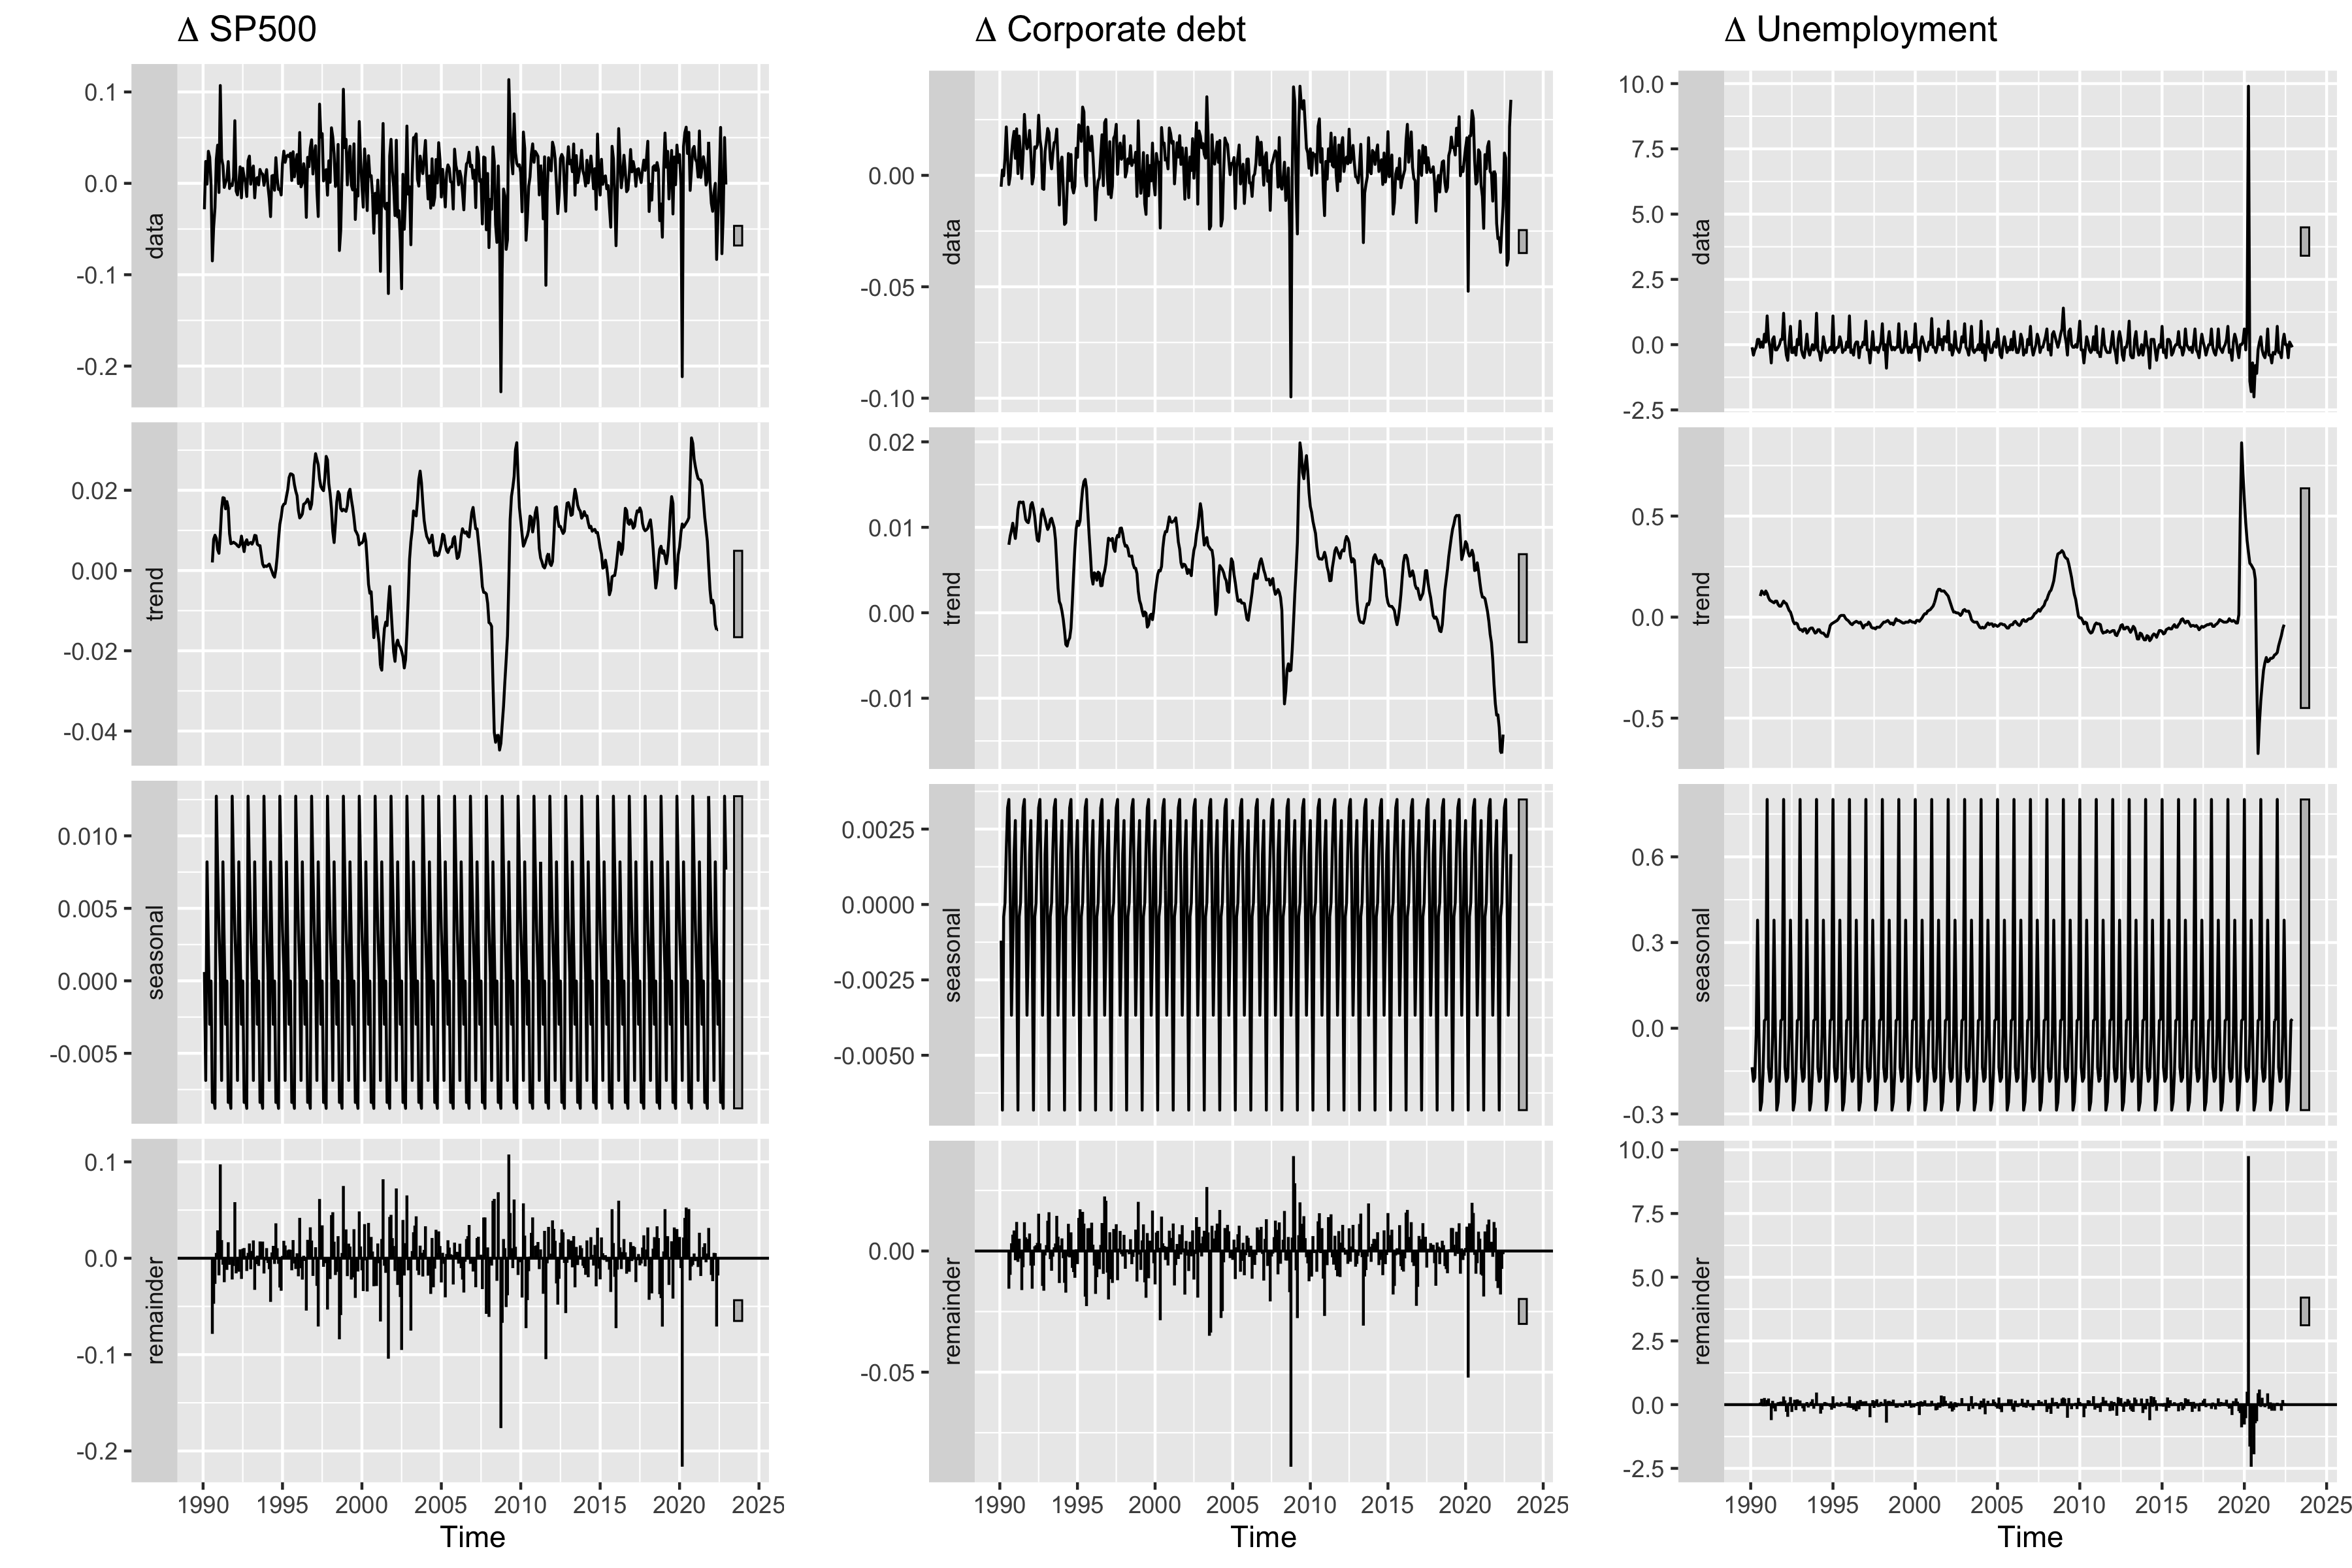
\includegraphics[width = 0.75\textwidth]{IMAGES/decomposition_iii_deltas.png}
    \caption{Decomposition of the series in deltas}
\end{figure}

\subsection{Check stationarity of the series in deltas if UR in levels}

To conclude that the previous three series are indeed I(1), we need to check that the series of their first differences are stationary (i.e. the series in deltas). 
We perform the same ADF procedure to test these transformed series. 


% Table created by stargazer v.5.2.3 by Marek Hlavac, Social Policy Institute. E-mail: marek.hlavac at gmail.com
% Date and time: Mon, Dec 11, 2023 - 23:21:57
\begin{table}[!htbp] \centering 
  \caption{ADF test - 1st regression with drift, deterministic trend and stochastic trend for series in deltas} 
  \label{tab:adfdeltas_hyp} 
\begin{tabular}{@{\extracolsep{5pt}} cccccccc} 
\\[-1.8ex]\hline 
\hline \\[-1.8ex] 
 & d\_gdp & d\_dpi & d\_rate & d\_splong & CV 1pct & CV 5pct & CV 10pct \\ 
\hline \\[-1.8ex] 
tau3 & $$-$10.437$ & $$-$19.070$ & $$-$7.107$ & $$-$13.317$ & $$-$3.980$ & $$-$3.420$ & $$-$3.130$ \\ 
phi2 & $36.317$ & $121.228$ & $16.895$ & $59.110$ & $6.150$ & $4.710$ & $4.050$ \\ 
phi3 & $54.473$ & $181.842$ & $25.327$ & $88.665$ & $8.340$ & $6.300$ & $5.360$ \\ 
\hline \\[-1.8ex] 
\end{tabular} 
\end{table} 


Table \ref{tab:adfdeltas_hyp} reports the test results in the first specification of the ADF test. 
We easily see that all the $t_\gamma$ (the statistic on tau3) are sufficiently negative to reject H0 and conclude that none of the differentiated series has a UR. 
This is sufficient to conclude that the series on the Fed fund rate, on the returns of the S\&P500, and on the return of corporate debt are indeed \emph{integrated of order one}. 



    \subsection{Cyclical component}






\section{Canonical VAR model application}\label{sec:var}

% latex table generated in R 4.3.1 by xtable 1.8-4 package
% Tue Dec  5 14:47:20 2023
\begin{table}[ht]
\centering
\caption{Canonical VAR in levels - Identify order} 
\begin{tabular}{rrrrrrrrrrr}
  \hline
 & 1 & 2 & 3 & 4 & 5 & 6 & 7 & 8 & 9 & 10 \\ 
  \hline
AIC(n) & -10.01 & -10.56 & -10.59 & -10.73 & -10.88 & -10.87 & -10.93 & -11.01 & -11.00 & -10.98 \\ 
  HQ(n) & -9.96 & -10.48 & -10.47 & -10.57 & -10.68 & -10.64 & -10.66 & -10.71 & -10.66 & -10.60 \\ 
  SC(n) & -9.89 & -10.35 & -10.29 & -10.33 & -10.38 & -10.29 & -10.25 & -10.25 & -10.14 & -10.03 \\ 
  FPE(n) & 0.00 & 0.00 & 0.00 & 0.00 & 0.00 & 0.00 & 0.00 & 0.00 & 0.00 & 0.00 \\ 
   \hline
\end{tabular}
\end{table}



% Table created by stargazer v.5.2.3 by Marek Hlavac, Social Policy Institute. E-mail: marek.hlavac at gmail.com
% Date and time: Wed, Dec 13, 2023 - 20:23:41
\begin{table}[!htbp] \centering 
  \caption{Level VAR - Estimation} 
  \label{tab:est_var_level} 
\small 
\begin{tabular}{@{\extracolsep{5pt}}lccc} 
\\[-1.8ex]\hline 
\hline \\[-1.8ex] 
 & \multicolumn{3}{c}{\textit{Dependent variable:}} \\ 
\cline{2-4} 
\\[-1.8ex] & \multicolumn{3}{c}{y} \\ 
 & splong & rate & gdp \\ 
\hline \\[-1.8ex] 
 splong.l1 & 0.186$^{***}$ & 0.011$^{***}$ & 0.447$^{**}$ \\ 
  & (0.051) & (0.004) & (0.205) \\ 
  gdp.l1 & 3.065$^{***}$ & 0.912$^{***}$ & 17.259$^{***}$ \\ 
  & (0.664) & (0.051) & (2.646) \\ 
  rate.l1 & $-$0.037$^{***}$ & 0.001 & 0.442$^{***}$ \\ 
  & (0.013) & (0.001) & (0.052) \\ 
  splong.l2 & $-$0.101$^{*}$ & $-$0.011$^{***}$ & $-$0.410$^{**}$ \\ 
  & (0.052) & (0.004) & (0.207) \\ 
  gdp.l2 & $-$1.076 & $-$0.034 & $-$13.109$^{***}$ \\ 
  & (0.899) & (0.069) & (3.580) \\ 
  rate.l2 & $-$0.009 & $-$0.005$^{***}$ & 0.102$^{*}$ \\ 
  & (0.014) & (0.001) & (0.058) \\ 
  splong.l3 & 0.084 & 0.008$^{**}$ & 0.290 \\ 
  & (0.053) & (0.004) & (0.211) \\ 
  gdp.l3 & 0.359 & $-$0.712$^{***}$ & $-$2.540 \\ 
  & (0.920) & (0.071) & (3.663) \\ 
  rate.l3 & 0.030$^{**}$ & 0.004$^{***}$ & 0.210$^{***}$ \\ 
  & (0.015) & (0.001) & (0.059) \\ 
  splong.l4 & 0.017 & 0.005 & $-$0.131 \\ 
  & (0.054) & (0.004) & (0.214) \\ 
  gdp.l4 & $-$1.164 & 0.620$^{***}$ & 14.481$^{***}$ \\ 
  & (0.947) & (0.073) & (3.772) \\ 
  rate.l4 & 0.011 & 0.001 & $-$0.134$^{**}$ \\ 
  & (0.015) & (0.001) & (0.062) \\ 
  splong.l5 & 0.103$^{*}$ & $-$0.004 & $-$0.340 \\ 
  & (0.054) & (0.004) & (0.215) \\ 
  gdp.l5 & 0.896 & $-$0.075 & $-$7.278$^{**}$ \\ 
  & (0.900) & (0.070) & (3.583) \\ 
  rate.l5 & 0.026$^{*}$ & $-$0.001 & 0.009 \\ 
  & (0.016) & (0.001) & (0.062) \\ 
  splong.l6 & $-$0.174$^{***}$ & 0.011$^{***}$ & $-$0.028 \\ 
  & (0.054) & (0.004) & (0.215) \\ 
  gdp.l6 & $-$0.236 & $-$0.296$^{***}$ & $-$1.729 \\ 
  & (0.832) & (0.064) & (3.313) \\ 
  rate.l6 & $-$0.043$^{***}$ & 0.001 & 0.121$^{*}$ \\ 
  & (0.015) & (0.001) & (0.061) \\ 
  splong.l7 & 0.056 & $-$0.002 & $-$0.238 \\ 
  & (0.054) & (0.004) & (0.216) \\ 
  gdp.l7 & $-$0.645 & 0.216$^{***}$ & 3.930 \\ 
  & (0.639) & (0.049) & (2.543) \\ 
  rate.l7 & 0.039$^{***}$ & $-$0.001 & 0.006 \\ 
  & (0.014) & (0.001) & (0.056) \\ 
  const & 0.002 & 0.001$^{***}$ & $-$0.062$^{***}$ \\ 
  & (0.005) & (0.0004) & (0.021) \\ 
  trend & $-$0.00001 & $-$0.00000 & 0.0001$^{*}$ \\ 
  & (0.00002) & (0.00000) & (0.0001) \\ 
 \hline \\[-1.8ex] 
Adjusted R$^{2}$ & 0.145 & 0.626 & 0.488 \\ 
Residual Std. Error (df = 365) & 0.034 & 0.003 & 0.134 \\ 
F Statistic (df = 22; 365) & 3.991$^{***}$ & 30.486$^{***}$ & 17.760$^{***}$ \\ 
\hline 
\hline \\[-1.8ex] 
\textit{Note:}  & \multicolumn{3}{r}{$^{*}$p$<$0.1; $^{**}$p$<$0.05; $^{***}$p$<$0.01} \\ 
\end{tabular} 
\end{table} 


\section{Cointegration theory}\label{sec:cointegration}




\section{Impulse Response Analysis}\label{sec:irf}
    \subsection{Canonical IRF}\label{sec:canonical_irf}


    \subsection{Structural IRF}\label{sec:structural_irf}



\section{Introduce non-linearities}\label{sec:nonlinearities}
    \subsection{Markov-switching model}\label{sec:markov}

    
    \subsection{STR model}\label{sec:str}



\section{Difference-in-Difference}
https://www.tidy-finance.org/r/difference-in-differences.html
    



\newpage
\begin{appendices}
    
    \section{Code - Data Cleaning} \label{sec:dta_clean}
        %\lstinputlisting[language=python]{DataCleaning.py}
        \lstinputlisting[language=Python]{DataCleaning.py}

\end{appendices}







\end{document}